\documentclass[margin=5mm, tikz]{standalone}
\usepackage[utf8x]{inputenc}
\usepackage{siunitx}
\usepackage{tikz}
\begin{document}
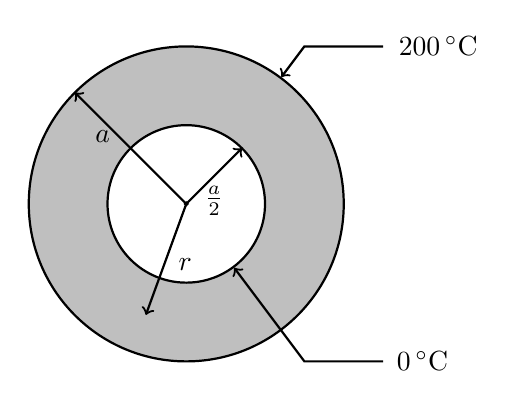
\begin{tikzpicture}[font=\normalsize]
	\tikzstyle{c1}=[circle,draw=black,fill=gray!50,thick, inner sep=0pt,minimum size=4cm]
	\tikzstyle{c2}=[circle,draw=black,fill=white,thick, inner sep=0pt,minimum size=2cm]
	\node (bola1) at (0, 0) [c1] {};
	\node (bola2) at (0, 0) [c2] {};
	\draw [fill] (0,0) circle (0.025);
	\draw [->, thick] (0, 0) -- (45:1) node [midway, below, pos= 0.5] {$\frac{a}{2}$};
	\draw [->, thick] (0, 0) -- (135:2) node [midway, below, pos = 0.75] {$a$};
	\draw [->, thick] (0, 0) -- (250:1.5) node [label={[xshift=0.5cm, yshift=0.3cm] $r$}] {};
	\draw [->, thick] (2.5, -2) -- (1.5, -2) -- (bola2);
	\node (valor1) at (3, -2) {$\SI{0}{\celsius}$};
	\draw [->, thick] (2.5, 2) -- (1.5, 2) -- (bola1);
	\node (valor2) at (3.2, 2) {$\SI{200}{\celsius}$};
	\end{tikzpicture}
\end{document}